\begin{figure}[ht]
   \centering
   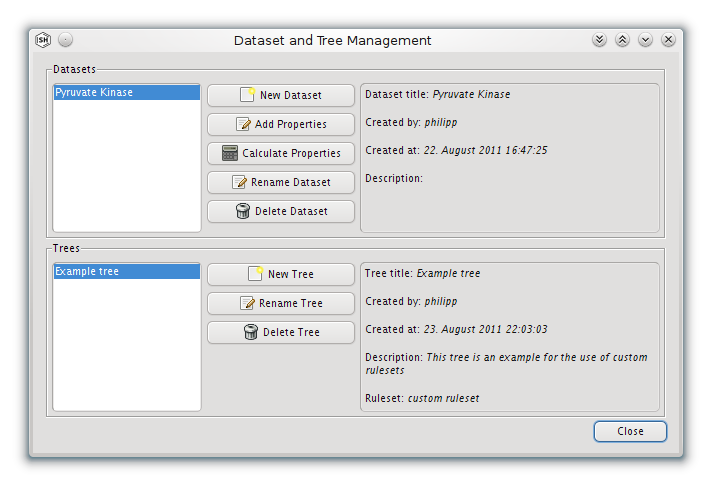
\includegraphics[width=\textwidth]{images/sh_dataset_management_dialog.png}
   \caption{Dataset Management Dialog}
   \label{fig:dataset_management}
\end{figure}

The \guidialog{Dataset Management Dialog} shown in \figref{fig:dataset_management} gives you the possibility to import, modify or delete the molecular data stored in \sh's internal database.
In \sh you can manage your projects by the use of datasets.
Each dataset consists of a set of molecules and a collection of properties for these molecules.
For each dataset you can generate an arbitrary number of scaffold trees using different generation rules.
You will later use the scaffold tree of your choice, to navigate through the molecules in the dataset.
In the following the actions you can execute on datasets and trees are explained.

\paragraph*{Actions on datasets}

\subparagraph*{New dataset}
To create a new dataset by importing chemical compound data, click on \gui{New Dataset} which opens the import wizard.
Read \secref{sec:scaffoldhunter:import} to get more information about the import process.

\subparagraph*{Add properties}
If you have an existing dataset and want to add some additional molecular properties (e.g. bioactivity information from a bio assay),
select the dataset from the list of datasets and click \gui{Add Properties}.
A wizard similar to the import wizard described in \secref{sec:scaffoldhunter:import} will appear.

\hintbox{Important}{Please note that you can only add additional properties to existing molecules.
For technical reasons it is not possible to add completely new molecules. If you try to do so, those molecules will simply be ignored.}

	
\subparagraph*{Calculate properties}
\sh gives you the opportunity to calculate additional properties (e.g. properties derived from the structure of a compound) for the molecules of a dataset.
Additionally, to enable some features like clustering molecules based on structural similarity, you may need to calculate fingerprint properties.
To calculate properties for a dataset, select the dataset from the list of datasets and click \gui{Calculate Properties}.
A dialog to create calculation tasks appears. Please read \secref{sec:scaffoldhunter:propertycalculation} to learn more about the calculation process.

\subparagraph*{Rename dataset}
If you created a dataset and would like to change its name or description, select the dataset from the list of datasets and click \gui{Rename Dataset}.
A rename dialog will appear.

\subparagraph*{Delete dataset}
If there is an existing dataset you don't need anymore, select it from the list of datasets and click \gui{Delete Dataset}.
A confirmation dialog will appear. If you confirm the deletion, the dataset and all trees in it will be deleted.

\warningbox{Warning}{\sh can be used by multiple users. If you are working on a database shared with other users, you will also destroy any work
done by other users on the dataset being deleted and the corresponding trees. First ensure nobody needs the dataset and the corresponding trees anymore.}

\paragraph*{Actions on trees}

\subparagraph*{New tree}
To create a new tree, select the dataset the tree should be generated for from the list of datasets and click \gui{New Tree}.
The tree generation dialog will appear. Read \secref{sec:scaffoldhunter:treegeneration} to learn more about how the tree generation process works.

\subparagraph*{Rename tree}
If you created a tree and would like to change its name or description, select the tree from the list of trees and click \gui{Rename Tree}.
A rename dialog will appear.

\subparagraph*{Delete tree}
If there is an existing tree you don't need anymore, select it from the list of trees on the left and click \gui{Delete Tree}.
A confirmation dialog will appear. If you confirm the deletion, the tree will be deleted.

\warningbox{Warning}{\sh can be used by multiple users. If you are working on a database shared with other users, you will also destroy any work
done by other users on the tree being deleted. First ensure nobody needs the tree anymore.}
